\scanpage{46}\mspage{8}
Soit $\vec\Delta$ une \inserted{ps-}droite \uline{orientée} ne passant pas
par $s$, alors l'orientation de $\vec\Delta$ en \unsure{définis|définit} une
de $I_s\subset S_\Delta$, i.e. un générateur $u_0$, noté
$(u_{\deleted{\unsure{\Delta}}s,\vec\Delta}$, de $Z_s^{\unsure{\prime|1}}=Z'_{s,\Delta}$. Si $\unsure{\nu_2|v_2|\nu_s}=2$, on prendra
$u_{s,\vec\Delta}$ la transposition de $I_s$ (de card 2), égal
ici à son inverse (i.e. \deleted{\unsure{$Z_s$}} ici $\operatorname{card} Z'_s=1$, et non 2).

On \deleted{doit} \deleted{doit} définir un $\vec u_{s,\vec\Delta}$ au dessus de
\deleted{\unsure{$u_s$}} $u_{s,\vec\Delta}$, ce qui fait (en exigeant que
soit une permutation circulaire) \inserted{un choix à déterminer parmi} $2^{\nu_s-1}$ \deleted{\unsure{de}}
possibilités \inserted{a priori}. (Le compte est bon, même pour
$\nu_s=2$). On est ramené ici, pour une ps-droite
$D_i$ passant par $s$, désignant par
$D_j$ son ``successeur'' pour $u_{s,\vec\Delta}$, à décrire
la bijection $\omega_i\xrightarrow{\sim}\omega_j$ induite par $\vec\Delta$,
donc pour le choix d'une
orientation sur \inserted{$D={}$} $D_i$, d'où
$\vec D_i$, il faut décrire
l'orientation correspondante de $D_j$ — en utilisant
l'orientation de $\vec\Delta$.

\figure{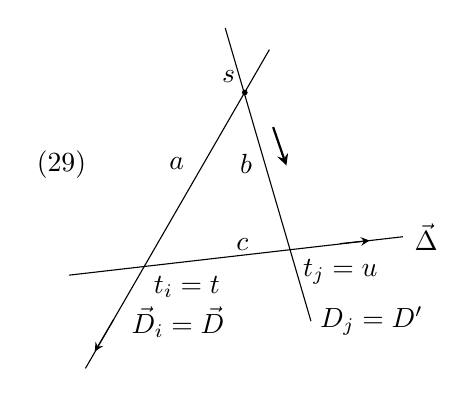
\begin{tikzpicture}[scale=.80,>=stealth]
\draw (-1.92,-2.40)--(1.00,2.66);
\draw (.30,3.00)--(1.66,-1.65);
\draw (-2.18,-.92)--(3.12,-.31);
\fill (.61,1.98) circle (.045) node[above left] {$s$};
\draw[->] (-1.47,-1.62)--(-1.77,-2.13);
\draw[->,thick] (1.06,1.43)--(1.27,.82);
\draw[->] (2.12,-.42)--(2.59,-.37);
\node at (-.47,.85) {$a$}; \node at (.63,.84) {$b$}; \node at (.57,-.44) {$c$};
\node[below right] at (-.99,-.78) {$t_i=t$}; \node[below right] at (1.38,-.51) {$t_j=u$};
\node at (-.45,-1.67) {$\vec D_i=\vec D$}; \node[right] at (1.65,-1.65) {$D_j=D'$};
\node[right] at (3.15,-.31) {$\vec\Delta$}; \node at (-2.30,.83) {(29)};
\end{tikzpicture}}
La figure montre que l'orientation à choisir sur
$D'=D_j$ est décrite par la condition que l'arête \inserted{$a$} \uline{joignant}
$s$ à $t=\varphi(i)$ (intersection de $D$ et $\deleted{\unsure{\leftarrow|\rightarrow}}\Delta$), dans le sens
de l'orientation \deleted{\unsure{donnée}} de $\vec D$, et celle $b$ joignant $s$ à $u=\varphi(j)$
(int. de $D'$ et $\Delta$) dans le sens de l'orientation cherchée de
$D'$, et enfin l'arête $c$ joignant $t$ à $u$ dans le sens
% archive sheet number: 45
